\documentclass[11pt,a4paper]{article}

% --- Essential Packages ---
\usepackage[utf8]{inputenc}
\usepackage[T1]{fontenc}
\usepackage{amsmath,amssymb,amsthm,mathtools}
\usepackage{geometry}
\geometry{margin=1in}
\usepackage{microtype}
\usepackage{booktabs}
\usepackage{enumitem}
\usepackage{tikz}
\usetikzlibrary{arrows.meta,positioning,shapes}
\usepackage[colorlinks=true,linkcolor=blue!70!black,citecolor=blue!70!black,urlcolor=blue!70!black]{hyperref}
\usepackage{cleveref}

% --- Theorem Environments ---
\theoremstyle{definition}
\newtheorem{definition}{Definition}[section]
\newtheorem{example}[definition]{Example}
\newtheorem{remark}[definition]{Remark}

\theoremstyle{plain}
\newtheorem{theorem}[definition]{Theorem}
\newtheorem{lemma}[definition]{Lemma}
\newtheorem{proposition}[definition]{Proposition}
\newtheorem{corollary}[definition]{Corollary}

% --- Document Metadata ---
\title{Bridge E-Hypergraphs: Specification}
\author{}
\date{\today}

\begin{document}

\maketitle

\section{Preliminaries: Signatures and Hypergraphs}

\begin{definition}[Monoidal Signature]
A \emph{(monoidal) signature} $\Sigma$ is given by a set of generating operations $c \colon n \to m$, where $n \in \mathbb{N}$ denotes the \emph{arity} (number of inputs) and $m \in \mathbb{N}$ denotes the \emph{co-arity} (number of outputs).
\end{definition}

\begin{definition}[Hypergraph]
A \emph{hypergraph} $G$ over a signature $\Sigma$ is a tuple $(V, E, s, t, l)$, where:
\begin{itemize}
    \item $V$ is a finite set of \emph{vertices};
    \item $E$ is a finite set of \emph{hyperedges};
    \item $s \colon E \to V^*$ is the \emph{source function}, mapping each hyperedge to an ordered sequence of input vertices;
    \item $t \colon E \to V^*$ is the \emph{target function}, mapping each hyperedge to an ordered sequence of output vertices;
    \item $l \colon E \to \Sigma$ is a \emph{labelling function} assigning each hyperedge a generator from $\Sigma$, respecting arities: for every $e \in E$, if $l(e) \colon n \to m$, then $|s(e)| = n$ and $|t(e)| = m$.
\end{itemize}
A hypergraph is called \emph{discrete} if $E = \emptyset$. An \emph{unlabelled hypergraph} is a tuple $(V, E, s, t)$ omitting the labelling function $l$.
\end{definition}

\section{E-Hypergraphs}

The combinatorial structure of an $E$-hypergraph formalises hierarchical equality graphs ($e$-graphs) by extending hypergraphs with a hierarchy of equivalence boxes ($e$-boxes) and a consistency relation separating distinct equivalent components within each box.

\begin{definition}[E-Hypergraph, Tiurin et al.~\cite{tiurin2024equivalence}]
\label{def:e-hypergraph}
An \emph{e-hypergraph} $G$ over a signature $\Sigma$ is a tuple
\[
G = (V, E, s, t, l, <, \smile),
\]
where:
\begin{itemize}
    \item $(V, E, s, t)$ is an unlabelled hypergraph;
    \item $l \colon E \to \Sigma + 1$ is a labelling function extended with an extra distinguished value $\bot \in 1$ in its codomain; an edge $e \in E$ is called \emph{hierarchical} (representing an $e$-box) if $l(e) = \bot$, and a \emph{base edge} otherwise;
    \item $<$ is a strict partial order on $V + E$, called the \emph{child relation}.
\end{itemize}

\paragraph{Hierarchical Notation.}
For any element $x \in V + E$:
\begin{itemize}
    \item The set of \emph{predecessors} (or \emph{parents}) of $x$ is denoted by
    \[
    [x) \coloneqq \{ x' \in V + E \mid x' < x \}.
    \]
    \item An element $x \in V + E$ is called \emph{top-level} if $[x) = \emptyset$.
    \item We write $e <^\mu x$ to denote that $e$ is the \emph{immediate parent} (predecessor) of $x$, meaning $e < x$ and there exists no $z \in V + E$ such that $e < z < x$. In this case, $x$ is called an \emph{immediate child} of $e$.
    \item An edge $e \in E$ is called \emph{maximal} if $\{ x' \in V + E \mid e < x' \} = \emptyset$ (i.e., it has no children in the hierarchy).
\end{itemize}

\paragraph{Hierarchy Axioms.}
The child relation $<$ must satisfy the following conditions:
\begin{enumerate}[label=(\arabic*)]
    \item \textbf{Parents are hierarchical edges:} each parent set $[x)$ contains exclusively hierarchical edges, i.e.,
    \[
    \forall x, p \in V + E, \quad p < x \implies (p \in E \land l(p) = \bot);
    \]
    \item \textbf{At most one immediate parent:} each element $x \in V + E$ has at most one immediate parent:
    \[
    \forall x, p_1, p_2 \in V + E, \quad (p_1 <^\mu x \land p_2 <^\mu x) \implies p_1 = p_2;
    \]
    \item \textbf{Maximal edges are not hierarchical:} all maximal edges carry a generator label:
    \[
    \forall e \in E, \quad (\forall x' \in V + E, \neg(e < x')) \implies l(e) \neq \bot;
    \]
    \item \textbf{Edges and incident vertices share parents:} for every hyperedge $e \in E$ and every vertex $v \in V$,
    \[
    v \in s(e) \implies (e' <^\mu e \iff e' <^\mu v),
    \]
    and similarly for target vertices:
    \[
    v \in t(e) \implies (e' <^\mu e \iff e' <^\mu v).
    \]
\end{enumerate}

\paragraph{Consistency Relation.}
The relation $\smile$ is the \emph{consistency relation}, defined as the union of a family of equivalence relations $\smile_p$ indexed by hierarchical parent edges $p \in E$ on each set of immediate children
\[
\{ x \in V + E \mid p <^\mu x \},
\]
satisfying:
\begin{enumerate}[label=(\alph*)]
    \item \textbf{Closed under connectivity:} if $v \in s(e)$ or $v \in t(e)$ with $p <^\mu v$ and $p <^\mu e$, then
    \[
    v \smile_p e;
    \]
    \item \textbf{Non-triviality:} for every parent $p$, $\smile_p$ does not collapse into the full indiscrete relation:
    \[
    \smile_p \neq (E_p + V_p) \times (E_p + V_p),
    \]
    where $V_p \coloneqq \{ v \in V \mid p <^\mu v \}$ and $E_p \coloneqq \{ e \in E \mid p <^\mu e \}$. That is, whenever an $e$-box $p$ has children, there exist at least two mutually inconsistent children ($x \not\smile_p y$), ensuring distinct alternative components.
\end{enumerate}

Given an $e$-hypergraph $G$, the corresponding \emph{underlying hypergraph} $G'$ is obtained by forgetting the hierarchy $<$ and consistency relation $\smile$.
\end{definition}

\section{The Subgraph Homomorphism Problem in E-Matching}

A natural categorical intuition for defining pattern matching is to view it as a strict homomorphism. When matching a flat pattern $P$ against a hierarchical E-hypergraph $G$, one might attempt to define a match as either a subgraph homomorphism of standard hypergraphs or a homomorphism in the category of E-hypergraphs. However, both approaches fundamentally fail when a pattern spans across e-box boundaries.

Consider a simple pattern $P$ consisting of two operations $A$ and $B$ connected in series by a single wire (vertex) $v$, such that $t(A) = s(B) = (v)$. Suppose we wish to match $P$ against a host E-hypergraph $G$ where $A$ belongs to an alternative within an e-box $E_1$, and $B$ belongs to an alternative within another e-box $E_2$, with the two e-boxes connected in series.

\begin{figure}[htbp]
\centering
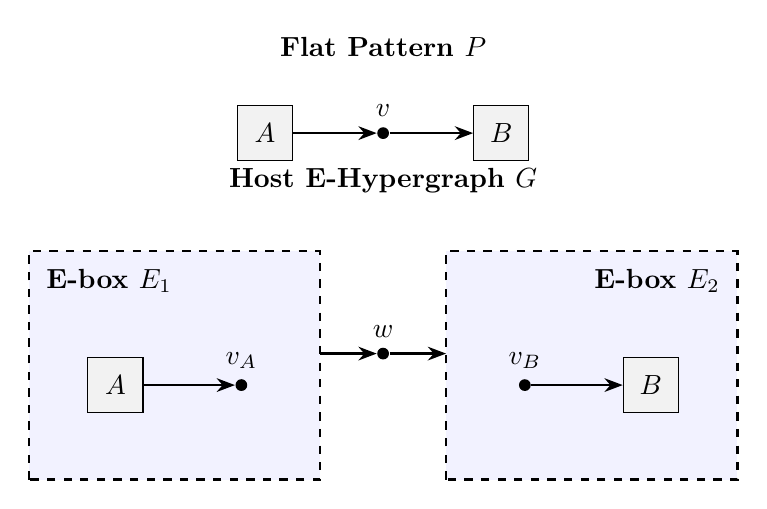
\begin{tikzpicture}[
  >={Stealth},
  node distance=1.5cm and 2cm,
  vertex/.style={circle, fill=black, inner sep=1.5pt},
  edgebox/.style={draw, rectangle, minimum height=0.7cm, minimum width=0.7cm, fill=gray!10},
  wire/.style={->, thick}
]

% Pattern P
\node (P_label) at (0, 2.3) {\textbf{Flat Pattern $P$}};
\node[edgebox] (A_P) at (-1.5, 1.2) {$A$};
\node[vertex, label=above:$v$] (v_P) at (0, 1.2) {};
\node[edgebox] (B_P) at (1.5, 1.2) {$B$};

\draw[wire] (A_P) -- (v_P);
\draw[wire] (v_P) -- (B_P);

% Host G
\begin{scope}[yshift=-2.6cm]
\node (G_label) at (0, 3.2) {\textbf{Host E-Hypergraph $G$}};

% E-box 1
\draw[dashed, thick, fill=blue!5] (-4.5, -0.6) rectangle (-0.8, 2.3);
\node[anchor=north west] at (-4.4, 2.2) {\textbf{E-box $E_1$}};
\node[edgebox] (A_G) at (-3.4, 0.6) {$A$};
\node[vertex, label=above:$v_A$] (v_A) at (-1.8, 0.6) {};
\draw[wire] (A_G) -- (v_A);

% E-box 2
\draw[dashed, thick, fill=blue!5] (0.8, -0.6) rectangle (4.5, 2.3);
\node[anchor=north east] at (4.4, 2.2) {\textbf{E-box $E_2$}};
\node[vertex, label=above:$v_B$] (v_B) at (1.8, 0.6) {};
\node[edgebox] (B_G) at (3.4, 0.6) {$B$};
\draw[wire] (v_B) -- (B_G);

% Top-level connection between e-boxes
\node[vertex, label=above:$w$] (w) at (0, 1.0) {};
\draw[wire] (-0.8, 1.0) -- (w);
\draw[wire] (w) -- (0.8, 1.0);

\end{scope}
\end{tikzpicture}
\caption{Topological disconnection in an E-hypergraph. In the pattern $P$, operations $A$ and $B$ directly share a vertex $v$. In the host E-hypergraph $G$, $A$ and $B$ are strictly isolated inside their respective e-boxes; only the e-boxes $E_1$ and $E_2$ themselves are connected via top-level vertex $w$.}
\label{fig:hom-counterexample}
\end{figure}

\paragraph{Topological Failure of Standard Subgraph Homomorphisms.}
In an E-hypergraph, Axiom~(4) (\emph{Edges and incident vertices share parents}) dictates that any vertex incident to an edge must share that edge's immediate parent:
\begin{itemize}
    \item Any target vertex $v_A \in t(A)$ must be an immediate child of $E_1$ ($E_1 <^\mu v_A$).
    \item Any source vertex $v_B \in s(B)$ must be an immediate child of $E_2$ ($E_2 <^\mu v_B$).
\end{itemize}
By Axiom~(2) (\emph{At most one immediate parent}), the child vertex sets of distinct e-boxes are strictly disjoint: no vertex can be a child of both $E_1$ and $E_2$. Furthermore, the connecting vertex $w$ between the two e-boxes is a top-level vertex ($[w) = \emptyset$), which means neither $A$ nor $B$ can be incident to $w$.

Consequently, as illustrated in \Cref{fig:hom-counterexample}, $A$ and $B$ are completely disconnected in the underlying hypergraph $G'$:
\[
t(A) \cap s(B) = \emptyset.
\]
A standard subgraph homomorphism $P \hookrightarrow G'$ requires mapping the vertex $v$ to a single shared vertex in $G'$ that connects $A$ and $B$. Because no such shared vertex exists, a strict topological match is impossible.

\paragraph{Failure of Categorical E-Hypergraph Homomorphisms.}
To preserve the hierarchical structure, one might instead attempt to lift $P$ to an E-hypergraph $P_E$ that mirrors $G$, placing $A$ inside a pattern e-box $E_{P1}$ and $B$ inside a pattern e-box $E_{P2}$, connected via $E_{P1} \to w \to E_{P2}$.

However, this construction fails categorically:
\begin{enumerate}
    \item \textbf{Violation of Non-Triviality:} A pattern represents a single concrete rewrite rule without internal alternatives. Thus, $E_{P1}$ and $E_{P2}$ would each contain only a single equivalence class (the singleton operation $A$ and $B$, respectively). By the \emph{Non-triviality} condition of \Cref{def:e-hypergraph}, every e-box with children must contain at least two mutually inconsistent children. Hence, $P_E$ is not a well-formed E-hypergraph.
    \item \textbf{Loss of Pattern Generality:} Even if trivial e-boxes were permitted, structuring $P$ to mirror the e-boxes of $G$ would mean a pattern could only match graphs that have the exact same hierarchy decomposition, destroying the ability of a flat pattern to match across arbitrary equivalence boundaries.
\end{enumerate}

Thus, matching cannot be formalized as a subgraph homomorphism (neither on the underlying hypergraph nor in the category of E-hypergraphs). Instead, an E-match is defined semantically with respect to the \emph{flattened extractions} of $G$. To make this operation computable without uncompressing the graph, an explicit representation of the interface between e-boxes and their contents is required.


\section{Bridge E-Hypergraphs}

As demonstrated in the previous section, the child alternatives inside an e-box are strictly isolated from the parent level by Axiom~(4) (\emph{Edges and incident vertices share parents}), preventing direct topological connections between child operations and surrounding context. 

To resolve this issue and make hierarchical graphs directly traversable, we introduce \emph{Bridge E-Hypergraphs}. The core mechanism is to introduce directed \emph{vertical hyperedges}, termed \emph{bridge edges}, that explicitly connect the external boundary of an e-box to the internal boundary of each child alternative:
\begin{itemize}
    \item An \emph{input bridge} $\mathrm{bridgeIn}(b, c)$ routes the external inputs of e-box $b$ vertically down into the internal inputs of choice $c$.
    \item An \emph{output bridge} $\mathrm{bridgeOut}(b, c)$ routes the internal outputs of choice $c$ vertically up into the external outputs of e-box $b$.
\end{itemize}

\begin{remark}[Comparison with Categorical Extended Interfaces]
In the foundational formulation of monoidal E-graphs by Tiurin et al.~\cite{tiurin2024equivalence}, the boundary between an e-box and its child contents is handled externally via categorical cospans of discrete interface graphs ($n \to n' \to G \leftarrow m' \leftarrow m$). While mathematically rigorous for DPO rewriting, this externalization splits the graph's topology between internal hyperedges $(s, t)$ and external morphism tables ($f_{\text{int}}, g_{\text{int}}$), creating significant overhead for graph algorithms. Bridge E-Hypergraphs internalize these interface mappings directly into the hypergraph as traversable vertical edges, making the graph self-contained and uniformly traversable by standard graph matching and extraction algorithms.
\end{remark}

\subsection{Computational Structure}

Separating computable data from logical invariants allows algorithms (such as pattern matching and extraction) to run on a concrete structure without incurring proof overhead.

\begin{definition}[Edge Kinds]
Given an edge set $E$, a signature $\Sigma$, and a set of choice identifiers $\mathcal{C}$, the set of \emph{edge kinds} $\mathrm{Kind}(E, \mathcal{C}, \Sigma)$ consists of:
\begin{itemize}
    \item $\mathrm{base}(\sigma)$ for $\sigma \in \Sigma$: standard operation edges;
    \item $\mathrm{ebox}$: hierarchical equivalence boxes;
    \item $\mathrm{bridgeIn}(b, c)$ for $b \in E, c \in \mathcal{C}$: an input bridge routing external inputs of e-box $b$ to choice $c$;
    \item $\mathrm{bridgeOut}(b, c)$ for $b \in E, c \in \mathcal{C}$: an output bridge routing internal outputs of choice $c$ to external outputs of e-box $b$.
\end{itemize}
\end{definition}

\begin{definition}[Bridge Graph]
A \emph{Bridge Graph} over signature $\Sigma$ and choice set $\mathcal{C}$ is a tuple
\[
G = (V, E, s, t, \mathrm{kind}, \mathrm{anchor}),
\]
where:
\begin{itemize}
    \item $(V, E, s, t)$ is an unlabelled hypergraph;
    \item $\mathrm{kind} \colon E \to \mathrm{Kind}(E, \mathcal{C}, \Sigma)$ classifies each hyperedge;
    \item $\mathrm{anchor} \colon E \times \mathcal{C} \to V + E$ maps each e-box and choice identifier to a canonical representative element (acting as a functional Union-Find root for the choice).
\end{itemize}
\end{definition}

\subsection{Bridge Graph Laws}

A Bridge Graph $G$ is called a \emph{valid Bridge E-Hypergraph} if there exist a strict partial order $<$ (child hierarchy) and a family of consistency equivalence relations $\smile_p$ satisfying the following laws:

\begin{enumerate}[label=\textbf{L\arabic*.}]
    \item \textbf{Hierarchy Foundations:}
    \begin{itemize}
        \item \emph{Parents are E-Boxes:} If $p < x$, then $p \in E$ and $\mathrm{kind}(p) = \mathrm{ebox}$.
        \item \emph{Unique Immediate Parent:} If $p_1 <^\mu x$ and $p_2 <^\mu x$, then $p_1 = p_2$.
        \item \emph{Maximal Edges:} If an edge $e$ has no children, then $\mathrm{kind}(e) \neq \mathrm{ebox}$.
    \end{itemize}

    \item \textbf{Scope Preservation (Bridge Exemption):}
    For all non-bridge edges $e \in E$, every incident vertex shares the immediate parent of $e$:
    \[
    \forall v \in s(e) \cup t(e), \quad (p <^\mu e \iff p <^\mu v).
    \]
    (Bridge edges are explicitly exempt, as they span across hierarchy levels).

    \item \textbf{Anchor Validity:}
    If an e-box $b$ has a bridge edge for choice $c$, the corresponding anchor is an immediate child:
    \[
    b <^\mu \mathrm{anchor}(b, c).
    \]

    \item \textbf{Interface Alignment (Vertical Boundary Routing):}
    For any bridge edge $e$ associated with e-box $b$ and choice $c$:
    \begin{itemize}
        \item If $\mathrm{kind}(e) = \mathrm{bridgeIn}(b, c)$, then:
        \[
        s(e) = s(b), \quad |t(e)| = |s(b)|, \quad t(e) \text{ has no duplicates}, \quad \forall v \in t(e), \; b <^\mu v.
        \]
        Furthermore, $t(e)$ represents pure inputs: no child edge $e' <^\mu b$ consistent with choice $c$ can have any vertex in $t(e)$ as a target ($t(e) \cap t(e') = \emptyset$).
        
        \item If $\mathrm{kind}(e) = \mathrm{bridgeOut}(b, c)$, then:
        \[
        t(e) = t(b), \quad |s(e)| = |t(b)|, \quad s(e) \text{ has no duplicates}, \quad \forall v \in s(e), \; b <^\mu v.
        \]
        Furthermore, $s(e)$ represents pure outputs: no child edge $e' <^\mu b$ consistent with choice $c$ can have any vertex in $s(e)$ as a source ($s(e) \cap s(e') = \emptyset$).
    \end{itemize}

    \item \textbf{Choice Consistency:}
    All internal ports of a bridge edge are consistent with the designated anchor:
    \[
    \forall v \in t(\mathrm{bridgeIn}(b, c)), \quad v \smile_b \mathrm{anchor}(b, c),
    \]
    \[
    \forall v \in s(\mathrm{bridgeOut}(b, c)), \quad v \smile_b \mathrm{anchor}(b, c).
    \]

    \item \textbf{Exhaustiveness and Uniqueness:}
    For every e-box $b$ and every child alternative, there exists a unique $\mathrm{bridgeIn}$ and a unique $\mathrm{bridgeOut}$ edge connecting to that alternative. Distinct choices have mutually inconsistent anchors.

    \item \textbf{Bridge Pairing:}
    Every input bridge $\mathrm{bridgeIn}(b, c)$ has a corresponding output bridge $\mathrm{bridgeOut}(b, c)$, and vice versa.
\end{enumerate}

\begin{thebibliography}{9}
\bibitem{tiurin2024equivalence}
Aleksei Tiurin, Chris Barrett, Dan~R. Ghica, and Nick Hu.
\newblock Equivalence Hypergraphs: DPO Rewriting for Monoidal E-Graphs.
\newblock \emph{arXiv preprint arXiv:2406.15882v2}, 2025.
\end{thebibliography}

\end{document}
